\doublespacing
\allowdisplaybreaks
\chapter{A new algorithm}
Our new algorithm to compute the tree edit distance is introduced in this chapter. It is implemented in C++. The new algorithm consists of two main steps: finding the root-leaf decomposition path and bottom-down enumeration for distance computation.
\section{Finding the Optimal Root-leaf Decomposition Path}
\subsection{Main Idea}
The heavy path decomposition can be seen as a greedy strategy which usually leads to a local optimum. However, a dynamic programming method can be applied to find the global optimum, which saves time complexity in each actual runs. To find the global optimal path of a tree, each possible paths is quantified and the path with the least number of sub-problems are selected to decompose the tree.
\subsection{Relevant Leftmost Forest and Relevant Rightmost Forest}

Two categories of decomposition strategies are introduced in Chapter 2. The one is path decomposition and the other is full decomposition. To quantify the cost of each paths, the actual number of sub-forests resulting from path decomposition and full decomposition is the prerequisite. Relevant leftmost forests, relevant rightmost forests and relevant special forests are first introduced by Dulucq ~\cite{dulucq2005decomposition}.

\begin{definition}
(Relevant leftmost forests)
Let T be a tree. The set of leftmost sub-forests of T is the least set satisfying, 
\begin{itemize}
\item for each node i of T, T(i) is the leftmost forest,
\item if $t \comp l(g)$ is a leftmost sub-forest, then $t \comp g$ is the leftmost sub-forest too.
\end{itemize}
\end{definition}

Symmetrically, we have relevant rightmost forests.

\begin{definition}
(Relevant rightmost forests)
Let T be a tree. The set of rightmost sub-forests of T is the least set satisfying,
\begin{itemize}
\item for each node i of T, T(i) is the rightmost forest,
\item if $l(g) \comp t$ is a rightmost sub-forest, then $g \comp t$ is the rightmost sub-forest too.
\end{itemize}
\end{definition}

\begin{definition}
(Relevant special forests)
Let T be a tree. The set of special forest is the set of relevant sub-forest resulting from the full decomposition.
\end{definition}

\begin{notation}
Let T be a tree,
\begin{itemize}
\item $\#left(T)$ denotes the number relevant leftmost forests.
\item $\#right(T)$ denotes the number of relevant rightmost forest.
\item $\#spec(T)$ denotes the number of relevant special forest.
\end{itemize}
\end{notation}

\subsection{Number of Relevant Forests For a Tree}

We define $R(T)$ as the set of relevant sub-forests in the tree T. Let T is the tree of the form $l(g)$, where $l$ is the root of the tree, and $g$ is the forest under the root. According to the Equation 2.2, we have the Lemma 3.1.1.

\begin{lemma}
$R(T) = R(l(g)) = \{l(g)\} \cup R(g)$, no matter what the direction is.
\end{lemma}

\begin{proof}
Straightforward implication of the Equation 2.2.
\end{proof}

We define $R(F)$ as the set of relevant sub-forest in the forest F. If we consider the left decomposition, F can be the form $l(g) \comp t$, where $l(g)$ be the leftmost tree, and $t$ be the rest of the forest. On the contrary, F can also be of the form $t \comp l(g)$, where $l(g)$ be the rightmost tree, and $t$ be the rest of the forest. Then we have the Lemma 3.1.2.

\begin{lemma}
\begin{equation*}
R(F) = R(l(g) \comp t) = {l(g) \comp t} \cup R(g \comp t) \cup R(l(g)) \cup R(t),\ if\ the\ direction\ is\ left.
\end{equation*}
\begin{equation*}
R(F) = R(t \comp l(g)) = {t \comp l(g)} \cup R(t \comp g) \cup R(l(g)) \cup R(t),\ if\ the\ direction\ is\ right.
\end{equation*}
\end{lemma}
\begin{proof}
Straightforward implication of the Equation 2.3.
\end{proof}

Given a decomposition strategy, the number of relevant sub-forests is a measure of the complexity of the associated edit distance algorithm. To qualify the sub-problems, we denote $\#rel$ the number of relevant forests.

\begin{lemma}
The number of relevant sub-forests of tree F with respect to a root-leaf path is equal to the
number of nodes in F.
\end{lemma}
\begin{proof}
The proof is by induction on the size of F.

Basis: by the definition of path decomposition, $\left\vert F \right\vert = 1$, then $\mathcal{F} = 1$, which is consistent with the Lemma.

Induction: We assume that $\left\vert F_k \right\vert = k$ holds for forest $F_k$ of size k. Then for the forest $F_{k+1}$ of size $k + 1$, by the definition of path decomposition, we have 
\begin{align*}
\left\vert \mathcal{F}(F_{k+1}) \right\vert &= \left\vert \{F_{k+1}\} \cup \mathcal{F}(F_{k+1}-v) \right\vert \\ 
&= 1 + \left\vert \mathcal{F}(F_{k+1} - v) \right\vert \\
&= 1 + k\\
\end{align*}
This concludes the proof.
\end{proof}

\begin{lemma}
The number of relevant sub-forests produced by a recursive path decomposition of tree T with root-leaf path partitioning is the sum of the sizes of all the relevant sub-trees in the recursive decomposition. Let $\Gamma(T)$ be the set of sub-trees partitioned by a root-leaf path.
\begin{equation*}
\left\vert \mathcal{F}(T) \right\vert = \sum_{T' \in \Gamma(T)}\left\vert T' \right\vert
\end{equation*}
\end{lemma}
\begin{proof}
From the definition of the path decomposition and Lemma 3.1.3.
\end{proof}


\begin{remark}
Let T be a tree,
\begin{equation*}
\#right(T) = \sum(\left\vert T(i) \right\vert, i \in T) - \sum(\left\vert T(j) \right\vert,\ j\ is\ a\ rightmost\ child).
\end{equation*}
\begin{equation*}
\#left(T) = \sum(\left\vert T(i) \right\vert, i \in T) - \sum(\left\vert T(j) \right\vert,\ j\ is\ a\ leftmost\ child).
\end{equation*}
\end{remark}

\begin{lemma}
Let T be a forest of size $n$.
\begin{equation*}
\#spec(T) = \frac{n(n+3)}{2} - \sum_{i \in T}\left\vert T(i) \right\vert
\end{equation*}
\end{lemma}
\begin{proof}
The proof is by induction of the size n.

Basis: if $n=0$, then $\#spec(T) = 0$ always hold.

Induction: if $n > 0$, then $T = l(g) \comp t$. We assume that the sub-forest of T ($g \comp t$) , whose size is $n - 1$, satisfies the induction hypothesis. Therefore, we have
\begin{equation*}
\#spec(g \comp t) = \frac{(n-1)(n+1)}{2} - \sum_{i \in g \comp t}\left\vert g \comp t(i) \right\vert
\end{equation*}
Since $g \comp t$ is a sub-forest of T, this implies
\begin{equation*}
\#spec(g \comp t) = \frac{(n-1)(n+1)}{2} - \sum_{i \in g \comp t}\left\vert F(i) \right\vert
\end{equation*}
By definition of the full decomposition, the set of special forest of T consists of two kinds of sub-forests:
\begin{itemize}
\item those containing the node $l$, which gives $\left\vert t \right\vert + 1$ sub-forests.
\item those not containing the node $l$, which gives $\#spec(g \comp t)$ sub-forests.
\end{itemize}
Then we have
\begin{equation*}
\#spec(T) = \left\vert t \right\vert + 1 + \#spec(g \comp t)
\end{equation*}
Note that $\left\vert t \right\vert + 1$ can be written as $n - \left\vert l(g) \right\vert + 1$
 
It follows that 
\begin{align*}
\#spec(F) &= n - \left\vert l(g) \right\vert + 1 + \frac{(n - 1)(n + 2)}{2} - \sum_{i \in g \comp t}\left\vert F(i) \right\vert \\
&= n + 1 + \frac{(n - 1)(n + 2)}{2} - \sum_{i \in F}\left\vert F(i) \right\vert \\
&= \frac{n(n+3)}{2} - \sum_{i \in F}\left\vert F(i) \right\vert\\
\end{align*}
This concludes the proof.
\end{proof}
\subsection{Number of Relevant forests for a Pair of Trees}
With the analysis of the number of relevant forests for a tree resulting from the path decomposition and the full decomposition, we are now able to look for the total number of the relevant forest for a pair of trees. Given a pair of trees $T_1$ and $T_2$ provided with the root-leaf path for $T_1$, it appears that all relevant forests of $T_1$ fall within three categories:
\begin{itemize}
\item those that are compared with all rightmost forests of $T_2$,
\item those that are compared with all leftmost forests of $T_2$,
\item those that are compared with all special forests of $T_2$.
\end{itemize} 

For a tree with root-leaf path, the node on the path inherit sub-forests of another tree from its parent. Therefore, Let T be a tree provided with the root-leaf path, the status of a node in the tree can be separated into four categories depending on the direction and the heritage:
\begin{itemize}
\item Free node: the node is the root of T, or is not on the root-leaf path.
\item Left node: the node is on the root-leaf path and is the leftmost child of its parent, which inherit leftmost forests of another tree.
\item Right node: the node is on the root-leaf path and is the rightmost child of its parent, which inherit rightmost forests of another tree.
\item All node: the node is on the root-leaf path and is neither the leftmost child nor the rightmost child of its parent.
\end{itemize}

\begin{lemma}
Given a pair of trees $T_1$ and $T_2$ provided with the root-leaf path for $T_1$, and i be a free node of $T_1$:
\begin{enumerate}
\item if the direction of i is left, then $T_1(i)$ compared with all rightmost forests of $T_2$.
\item if the direction of i is right, then $T_1(i)$ compared with all leftmost forests of $T_2$.
\end{enumerate}
\end{lemma}
\begin{proof}
Proof by ~\cite{dulucq2005decomposition}
\end{proof}

\begin{lemma}
Given a pair of trees $T_1$ and $T_2$ provided with the root-leaf path for $T_1$, and i be a node of $T_1$ that is not free, and j be the parent of i:
\begin{enumerate}
\item if the direction of i is left, if i is the rightmost child of j and $T_1(j)$ is compared with all rightmost forests of $T_2$, then $T_1(i)$ is compared with all rightmost forests of $T_2$.
\item if the direction of i is right, if i is the leftmost child of j and $T_1(j)$ is compared with all leftmost forests of $T_2$, then $T_1(i)$ is compared with all leftmost forests of $T_2$.
\item otherwise $T_1(i)$ is compared with all special forests of $T_2$.
\end{enumerate}
\end{lemma}
\begin{proof}
Proof by ~\cite{dulucq2005decomposition}
\end{proof}
\begin{notation}
Let $A$ be a tree, $i$ be a node of $A$, and $j$ be the parent of $i$(if $i$ is not the root). Let $B$ be another tree, $i'$ be a node of $B$, and $j'$ be the parent of $i'$(if $i'$ is not the root). The root-leaf path can on either tree.
\begin{itemize}
\item $Free(A(i), B(i'))$ the set of $R(A, B) \cap (A(i), B(i'))$ if $i$ and $i'$ is free
\item $RightA(A(i), B(i'))$ the set of $R(A, B) \cap (A(i), B(i'))$ if $i$ is on the root-leaf path and is the rightmost child of $j$
\item $RightB(A(i), B(i'))$ the set of $R(A, B) \cap (A(i), B(i'))$ if $i'$ is on the root-leaf path and is the rightmost child of $j'$
\item $LeftA(A(i), B(i'))$ the set of $R(A, B) \cap (A(i), B(i'))$ if $i$ is on the root-leaf path and is the leftmost child of $j$
\item $LeftB(A(i), B(i'))$ the set of $R(A, B) \cap (A(i), B(i'))$ if $i'$ is on the root-leaf path and is the leftmost child of $j'$
\item $AllA(A(i), B(i'))$ the set of $R(A, B) \cap (A(i), B(i'))$ if $i$ is on the root-leaf path and neither the rightmost nor leftmost child of $j$
\item $AllB(A(i), B(i'))$ the set of $R(A, B) \cap (A(i), B(i'))$ if $i'$ is on the root-leaf path and neither the rightmost nor leftmost child of $j'$ 
\end{itemize}
\end{notation}
With the notation, we are now able to formulate the main result of the section, which gives the total number of relevant forests for a root-leaf path.
\begin{theorem}
Let(A, B) be a pair of trees, and the root-leaf is on either tree.
\begin{enumerate}
\item if A and B is reduced to a single node 
\begin{align*}
Free(A, B) &= LeftA(A, B) = LeftB(A, B)\\
&= RightA(A, B) = RightB(A, B)\\
&= AllA(A, B) = AllB(A, B) = 1\\
\end{align*}
\item if A is reduced to a single node, and B is a tree of the form $B = l(B')$, where $B'$ is a sub-tree.
\begin{eqnarray*}
&&Free(A, B) = min \begin{cases}
			RightB(A, B') + \#right(A)\\
			LeftB(A, B') + \#left(A)\\
			\end{cases}\\
&&LeftA(A, B) = \#left(B)\\
&&LeftB(A, B) = LeftB(A, B') + \#left(A)\\
&&RightA(A, B) = \#right(B)\\
&&RightB(A, B) = RightB(A, B') + \#right(B)\\
&&AllA(A, B) = \#spec(B)\\
&&AllB(A, B) = AllB(A, B') + \#spec(A)\\
\end{eqnarray*}
\item if A is reduced to a single node, and B is a tree of the form $B = l(B_1 \comp \cdots \comp B_n)$, where $B_1, B_2 \cdots B_n$ are sub-trees.
\begin{eqnarray*}
&&Free(A, B) = min \begin{cases}
			\sum_{i>1}Free(A, B_i) + LeftB(A, B_1) + \#left(A) * \left\vert  B - B_1 \right\vert \\
			\sum_{i \neq j}Free(A, B_i) + AllB(A, B_j) \\
			\ \ \ \ \ + min \begin{cases}
			\#right(A) * (1 + \left\vert B_1 \comp \cdots \comp B_{j-1} \right\vert) + \#spec(A) * (\left\vert B_{j+1} \comp \cdots \comp B_n \right\vert) \\
			\#left(A) * (1 + \left\vert B_n \comp \cdots \comp B_{j+1} \right\vert) + \#spec(A) * (\left\vert B_1 \comp \cdots \comp B_{j-1} \right\vert) \\
			\end{cases}\\
			\sum_{i < n}Free(A, B_i) + RightB(A, B_n) + \#right(A) * \left\vert B - B_n \right\vert \\
			\end{cases}\\
&&LeftA(A, B) = \#left(B)\\
&&LeftB(A, B) = \sum_{i > 1}Free(A, B_i) + LeftB(A, B_1) + \#left(A) * (\left\vert B - B_1 \right\vert)\\
&&RightA(A, B) = \#right(B)\\
&&RightB(A, B) = \sum_{i < n}Free(A, B_i) + RightB(A, B_n) + \#left(B) * (\left\vert B - B_n \right\vert)\\
&&AllA(A, B) = \#spec(B)\\
&&AllB(A, B) = min \sum_{i \neq j}Free(A, B_i) + AllB(A, B_j) + \#spec(A) * (\left\vert A - A_j \right\vert)\\
\end{eqnarray*}
\item if A is a tree of the form $A = l(A')$, and B is a tree of the form $B = l(B_1 \comp \cdots \comp B_n)$, where $B_1, B_2 \cdots B_n$ are sub-trees.
\begin{eqnarray*}
&&Free(A, B) = min \begin{cases}
			Free(A', B) + min \begin{cases}
			\#left(B) \\
			\#right(B) \\
			\end{cases}\\
			\sum_{i>1}Free(A, B_i) + LeftB(A, B_1) + \#left(A) *(\left\vert B - B_1 \right\vert)\\
			\sum_{i \neq j}Free(A, B_i) + AllB(A, B_1) \\
			\ \ \ \ + min \begin{cases}
			\#right(A) * (1 + \left\vert B_1 \comp \cdots \comp B_{j-1} \right\vert) + \#spec(A) * (\left\vert B_{j+1} \comp \cdots \comp B_n \right\vert)\\
			\#left(A) * (1 + \left\vert B_n \comp \cdots \comp B_{j+1} \right\vert) + \#spec(A) * (\left\vert B_1 \comp \cdots \comp B_{j-1} \right\vert)\\
			\end{cases}\\
			\sum_{i<n}Free(A, B_i) + RightB(A, B_n) + \#right(A) * (\left\vert B - B_n \right\vert)\\  
			\end{cases}\\
&&LeftA(A, B) = LeftA(A', B) + \#left(B)\\
&&LeftB(A, B) = \sum_{i>1}Free(A, B_i) + LeftB(A, B_1) + \#left(A)* (\left\vert B - B_1 \right\vert)\\
&&RightA(A, B) = RightA(A', B) + \#right(B)\\
&&RightB(A, B) = \sum_{i<n}Free(A, B_i) + RightB(A, B_n) + \#right(A) * (\left\vert B - B_n \right\vert)\\
&&AllA(A, B) = AllA(A', B) + \#spec(B)\\
&&AllB(A, B) = min \sum_{i \neq j}Free(A, B_i) + AllB(A, B_j) + \#spec(A) * (\left\vert B - B_j \right\vert)\\	
\end{eqnarray*}
\item if A is a tree of the form $A = l(A_1 \comp \cdots \comp A_n)$, and B is a tree of the form $B = l'(B_1 \comp \cdots \comp B_n)$
\begin{eqnarray*}
&&Free(A, B) = min \begin{cases}
			\sum_{i>1}Free(A_i, B) + LeftA(A_1, B) + \#left(B)*(\left\vert A - A_1 \right\vert) \\
			\sum_{i \neq j}Free(A_i, B) + AllA(A_j, B) \\
			\ \ \ \ + min\begin{cases}
			\#right(B) * (1 + \left\vert A_1 \comp \cdots \comp A_{j-1} \right\vert) + \#spec(B) * (\left\vert A_{j+1} \comp \cdots \comp A_n \right\vert) \\
			\#left(B) * (1 + \left\vert A_n \comp \cdots \comp A_{j+1} \right\vert) + \#spec(B) * (\left\vert A_1 \comp \cdots \comp A_{j-1} \right\vert) \\
			\end{cases}\\
			\sum_{i<n}Free(A_i, B) + RightA(A_n, B) + \#right(B)*(\left\vert A - A_n \right\vert) \\
			\sum_{i>1}Free(A, B_i) + LeftB(A, B_i) + \#left(A)*(\left\vert B - B_1 \right\vert) \\
			\sum_{i \neq j}Free(A, B_i) + AllB(A, B_j) \\
			\ \ \ \ + min\begin{cases}
			\#right(A) * (1 + \left\vert B_1 \comp \cdots \comp B_{j-1} \right\vert) + \#spec(A) * (\left\vert B_{j+1} \comp \cdots \comp B_n \right\vert)\\
			\#left(A) * (1 + \left\vert B_n \comp \cdots \comp B_{j+1} \right\vert) + \#spec(A) * (\left\vert B_1 \comp \cdots \comp B_n \right\vert) \\
			\end{cases}\\
			\sum_{i<n}Free(A, B_i) + RightB(A, B_n) + \#right(A)*(\left\vert B - B_n \right\vert)\\ 
			\end{cases}\\
&&LeftA(A, B) = \sum_{i>1}Free(A_i, B) + LeftA(A_1, B) + \#left(B) * (\left\vert A - A_1 \right\vert)\\
&&LeftB(A, B) = \sum_{i>1}Free(A, B_i) + LeftB(A, B_1) + \#left(A) * (\left\vert B - B_1 \right\vert)\\
&&RightA(A, B) = \sum_{i<n}Free(A_i, B) + RightA(A_n, B) + \#right(B) * (\left\vert A - A_n \right\vert)\\
&&RightB(A, B) = \sum_{i<n}Free(A, B_i) + RightA(A, B_n) + \#right(A) * (\left\vert B - B_n \right\vert)\\
&&AllA(A, B) = min \sum_{i \neq j}Free(A_i, B) + AllA(A_j, B) + \#spec(B) * (\left\vert A - A_j \right\vert)\\
&&AllB(A, B) = min \sum_{i \neq j}Free(A, B_i) + AllB(A, B_j) + \#spec(A) * (\left\vert B - B_j \right\vert)\\
\end{eqnarray*}
\end{enumerate}
\end{theorem}
\subsection{Dynamic Programming Implementation}
To compute the cost of each possible root-leaf paths, a dynamic programming way to implement is to define seven tables of size $n * m$ to store intermediate results, where $n$ and $m$ is the size of tree $A$ and tree $B$ respectively. For any pair of trees $(T_1, T_2)$, define dynamic programming tables $Free$, $RightA$, $RightB$, $LeftA$, $LeftB$, $AllA$ as well as $AllB$ indexed by nodes of tree $A$ and $B$. The definition of these seven tables borrowed from the Theorem 3.1.8. The algorithm loops over every pair of sub-trees in post-order of the nodes $i \in A$ and $j \in B$. At each step, the favorite node on the root-leaf path is chosen to be the child that minimizes the number of relevant forests.  For instance, if $A = l(A_1 \comp \cdots \comp A_n)$ and $B = l'(B_1 \comp \cdots \comp B_n)$ then, the favorite child is selected to be the root of the sub-tree in tree $A$  or $B$. The optimal root-leaf of each pairs of sub-trees can be built up by tracing back from table $Free(A, B)$.

\begin{lemma}
The time complexity of this pre-processing is in $\mathcal{O}(mn)$, where $m$ and $n$ is the size of tree $A$ and $B$ respectively.
\end{lemma}
\begin{proof}
Firstly, $\#right(A)$, $\#left(A)$ and $\#spec(A)$ are needed to compute. This can be made in $\mathcal{O}(m)$. Similarly, $\#right(B)$, $\#left(B)$ and $\#spec(B)$ can be computed in $\mathcal{O}(n)$. Next, we need to fill up seven array of the size $m * n$. Each cells stores the number relevant sub-forests of a pair of sub-trees in tree $A$ and $B$. The time to fill up the cell of each cell of node $i$ in the tree $A$ and node $j$ in the tree $B$ is proportional to the sum of the degree of $i$ and the degree of $j$. In other words, the time for the computation of each tables is in $\mathcal{O}(n\sum_{i \in A}deg(i) + m \sum_{j \in B}deg(j))$, that is in $\mathcal{O}(mn)$. 
\end{proof}

\section{Distance Computation in Bottom-up Fashion}
Once the optimal root-leaf path is set up, it is possible to compute the distance. 
\subsection{Double Roots Encoding}
We use root encoding to identify all sub-forests that can result from decomposing two trees using Equation 2.2 and 2.3.  
\begin{definition}
(Double roots encoding)
Let F be a forest, the root of the leftmost tree $lr(F)$ and the root of the rightmost tree $rr(F)$ be two nodes of forest F, $lr(F) \leq rr(F)$. The root encoding $F_{lr(F), rr(F)}$ defines a sub-forest of F with a set of nodes and edges. The set of nodes is defined as follows. Let x be nodes in the forest and  x succeeds $lr(F)$ in left-to-right pre-order and x succeeds $rr(F)$ in right-to-left pre-order.  
\begin{equation*}
N(F_{lr(F), rr(F)}) = \{lr(F), rr(F)\} \cup \{x\}
\end{equation*}
The edges set is defined as follows.
\begin{equation*}
E(F_{lr(F), rr(F)}) = \{(v, w) \in E(F) | v \in F_{lr(F), rr(F)} \cap w \in F_{lr(F), rr(F)}\}
\end{equation*}
\end{definition}

Figure 3.1 is an example of sub-forests of tree $G$ and their root encoding representation. The figure on the left is a sub-forest in G(black nodes) while the right on is a sub-tree. In the figures, the leftmost root and the rightmost root are marked with arrows. The left subscript of a node is its left-to-right and the right subscript its right-to-left pre-order. Take the left figure as an example, The left-to-right pre-order of the leftmost root is 2 and the right-to-left pre-order of rightmost root is 4. As shown in the right figure, if the right-to-left pre-order of the leftmost root is the same as the left-to-right pre-order of the rightmost root, the forest becomes a tree.

\begin{figure}
		\centering
		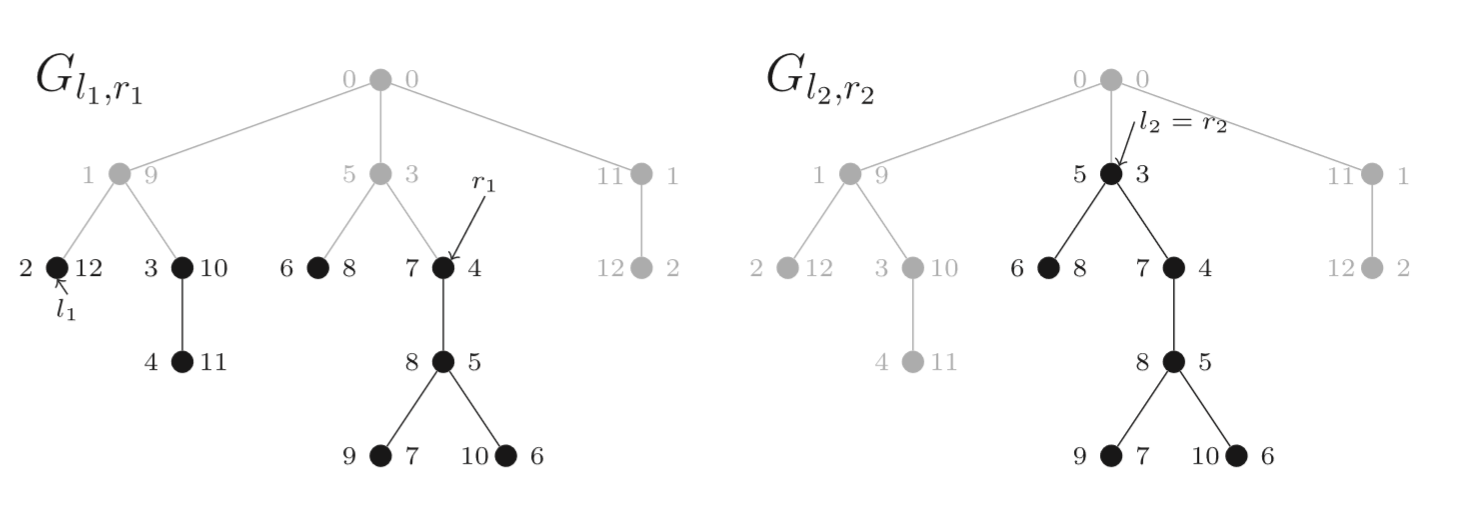
\includegraphics[width=14cm,clip]{Figures/RootEncoding}
		\label{Example subforests of tree G and their root encoding representation} 
		\caption{Example subforests of tree G and their root encoding representation~\cite{pawlik2015efficient}.}
\end{figure}
\subsection{Bottom-up Enumeration}
We presented the double root encoding for indexing sub-forests in the last section. In this section we make the use of this indexing scheme and present an algorithm for the enumeration of sub-forests pairs in bottom-up fashion.

The input of the algorithm are two trees $A$ and $B$ and a root-leaf path $\gamma$ of tree $A$. In algorithm 5, $p(v)$ is defined as the parent of the node $v$.
\IncMargin{1em}
\begin{algorithm}
  \caption{SUB\_FOREST\_PAIRS\_ENUMERATION}
  \SetKwInOut{Input}{inputs}
  \SetKwInOut{Output}{output}
  \SetKwData{TreeA}{$A$}
  \SetKwData{TreeB}{$B$}
  \SetKwData{RLP}{$\gamma$}
  \SetKwFunction{POSTORDER}{LR\_POSTORDER}{}{}

  \Input{\TreeA , \TreeB , \RLP}
  
  \ForEach{$node\ v\ \in\ \TreeA\ on\ the\ path\ from\ \epsilon\ to\ root$} { 
    $B' \gets B$\;
    $l_A^{last} \gets \varnothing$\;
    $l_A' \gets v$\;
  	\If{$\gamma\ is\ right\ or\ inner$} {
      \ForEach{$node\ r_B \in\ B\ in\ reverse\ right-to-left\ preorder$} { 
    	\If{$\gamma\ is\ right$} {   
    	  $l_A^{last} \gets p(v)$\;
    	  \lIf{$r_B\ is\ the\ rightmost\ child\ of\ its\ parent$} {
		     $B' \gets B(p(r_B))$  				
    	  }
    	  \lElse{
    		 $B' \gets \varnothing$
    	  }
    	  $r_A \gets v$\; 		
    	  }
    	  \ForEach{$node\ l_A \in\ left(A(p(v)), v) \cup l_A^{last}\ in\ reverse\ left-to-right\ preorder$} {
    	     \lIf{$l_A = p(v)$} {
			   $r_A \gets p(v)$				
    		  }
    		 \ForEach{$node\ l_B\ \in\ \{r_B\} \cup left(G, r_B)\ in\ reverse\ left-to-right\ preorder$} {
    			Compute forest-to-forest distance $d(l_A, r_A, l_B, r_B)$ as in Equation 2.3\;
    		  }
    		  $l_A' \gets l_A$\;
    		 }
    	  }	    	
    	}
     \If{$\gamma\ is\ left\ or\ inner$} {
     	\ForEach{$node\ l_B \in\ B\ in\ reverse\ right-to-left\ preorder$} {
     	  \If{$\gamma\ is\ left$} {
			\lIf{$l_B\ is\ the\ leftmost\ child\ of\ its\ parent$} {
			  $B' \gets B(p(l_B)$		
			}
			\lElse {
              $B' \gets \varnothing$		
			}
     	  }
     	  $l_A \gets l_A'$\;	
     	  \ForEach{$node\ r_A \in\ right(A(p(v)), v) \cup p(v)\ in\ reverse\ right-to-left\ preorder$} {
			\lIf{$r_A = p(v)$} {
				$l_A \gets p(v)$		
			}
			
			\ForEach{$node\ r_B \in\ l_B \cup right(B', l_B)\ in\ reverse\ right-to-left\ preorder$} {
				Compute forest-to-forest distance $d(l_A, r_A, l_B, r_B)$ as in Equation 2.3\;		
			}     	  
     	  }		     	
     	}
     }
    }
\end{algorithm}

The sub-problems are produced in nested loops and are nested as follows:$A(B(C(D)), B'(C'(D')))$. A relevant sub-forests pair is defined of the form $(l_A, r_A, l_B, r_B)$ using double roots encoding. Each loops enumerate one of these nodes. In the innermost loop, the distance for the relevant sub-forests pair is computed via Equation 2.2 and 2.3.

Loop A iterates bottom-up over the nodes of path $\gamma$ staring with a dummy leaf node $\epsilon$ which is appended to the leaf node of the path $\gamma$. The dummy is used for prevent the leaf node being treated as a special case. Figure 3.2 illustrates the order of processing nodes in loops A.

\begin{figure}
		\centering
		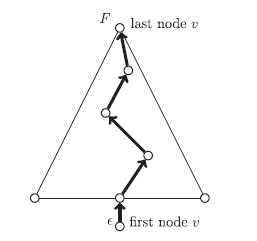
\includegraphics[width=4cm,clip]{Figures/loopA}
		\label{The order of processing nodes in loops A} 
		\caption{The order of processing nodes in loops A~\cite{pawlik2015efficient}.}
\end{figure}

Loop C enumerates the nodes to the left of path $\gamma$. The nodes set $left(A(p(v)), v)$ for a node enumerated in loop A is illustrated in Figure 3.3. Loop C(Figure 3.3(a)) defines the leftmost root node $l_A$ while the rightmost root node $r_A = v$ is defined by loop A. Symmetrically, loop C'(Figure 3.3(b)) iterates over the nodes from the set $right(A(p(v), v) \cup p(v)$ and defines the rightmost root node of the sub-forest, while the leftmost root node is the leftmost child of $p(v)$.

\begin{figure}
		\centering
		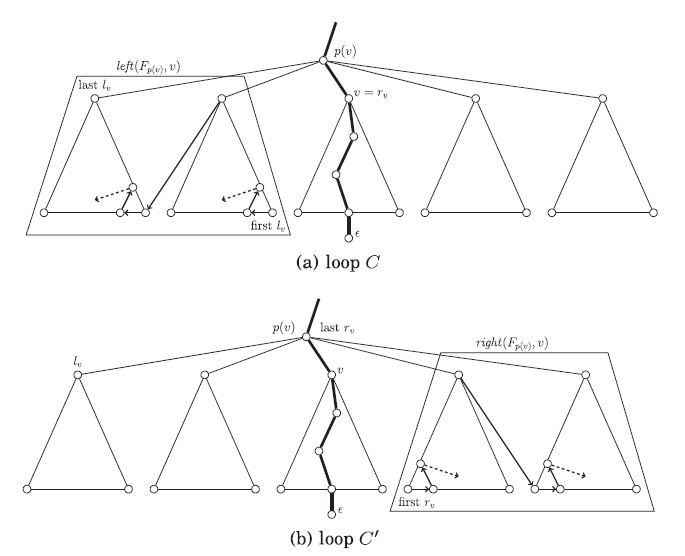
\includegraphics[width=10cm,clip]{Figures/loopCC}
		\label{The order of processing nodes in loop C and C'.} 
		\caption{The order of processing nodes in loop C and C'.~\cite{pawlik2015efficient}.}
\end{figure}

Loop B and loop D defines sub-forests of the tree $B$. The rightmost root node of sub-forest is iterates over all nodes of tree $B$ in reverse right-to-left preorder(Figure 3.4). After fixing the rightmost root node in loop B, the leftmost root node is iterated over all nodes to the left of leftmost root node in a specific sub-tree $B'$. 

\begin{figure}
		\centering
		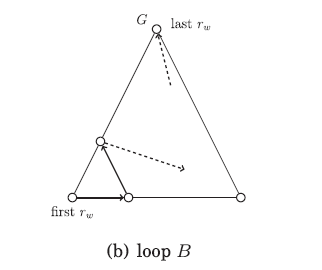
\includegraphics[width=6cm,clip]{Figures/loopB}
		\label{The order of processing nodes in loop B.} 
		\caption{The order of processing nodes in loop B.~\cite{pawlik2015efficient}.}
\end{figure}

\begin{figure}
		\centering
		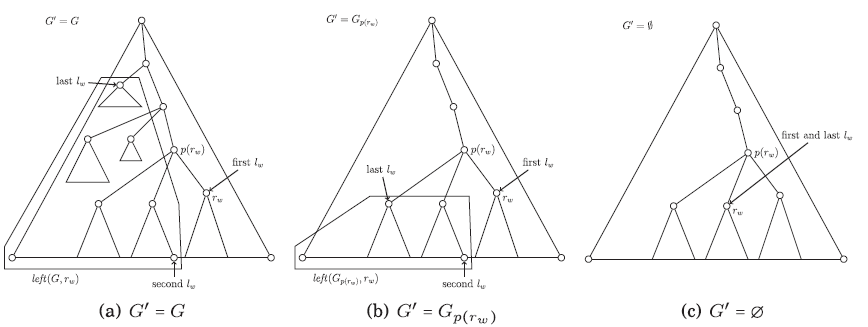
\includegraphics[width=14cm,clip]{Figures/loopD}
		\label{The order of processing nodes in loop D.} 
		\caption{The order of processing nodes in loop D.~\cite{pawlik2015efficient}.}
\end{figure}

The specific sub-tree $B'$ defines the set of nodes to be enumerated in loop D. The definition of $B'$ depends on the type of path $\gamma$ and the position of $r_B$ in B.
\begin{itemize}
\item Inner path $B' = B$(Figure 3.5(a))
\item Right path. If the rightmost root node $v$ is the rightmost child of its parent, then $B' = B(p(v))$(Figure 3.5(b)). Otherwise, $B' = \varnothing$(Figure 3.5(c)). 
\end{itemize}

Left paths are treated in loop B' and D', which are symmetric to loop B and D.

Algorithm 5 first enumerates the nodes to the left of the path then nodes to the right of the path in $A$. However, a symmetric version of Algorithm 5 goes on the other way: first iterates nodes to the right of the path then nodes to the right of the path. Since the directions of each nodes is not always the same, the symmetric version of  Algorithm 5 is included in our project as well.


\subsection{A Quadratic Space Complexity Implementation}
We have presented an algorithm for the enumeration of sub-forests pairs. It gives rise to two data structures:
\begin{itemize}
\item a permanent array D that stores the distance between a pair of sub-trees in two trees.
\item a temporary array F that stores the distance between a pair of sub-forests that are attached to the computation of a pair of sub-trees. 
\end{itemize}

Let $A$ and $B$ be two trees, and $\gamma$ be the root-leaf path on tree $A$. At the first glance, the array F requires cubic space, when the node on the root-leaf path is neither the leftmost child, nor the rightmost child, as the full decomposition of another tree is required in these cases.But it can be made quadratic with the introduction of two memorization tables: T and Q of sizes $\left\vert B \right\vert^2$ and $\left\vert A \right\vert$, where $A$ and $B$ are two trees.
\begin{itemize}
\item T stores the distance between a specific sub-forest in $A$ and each relevant sub-forests in $B$. 
\item Q stores the distance between each sub-forests of $A$ defined in loop C and a specific sub-forest in $G$, that is $G^{\comp}$
\end{itemize}

The tables T and Q are maintained in each loops C and C', which are needed in different calls of loops A and loops B(B').  In each loops A and B(B'), the intermediate results computed in the last loops are retrieved and is used for computation. Then, the new results are updated in T and Q for the next loop.

We now show how to retrieve intermediate result with the help of memorization tables $T$ and $Q$. Before we introduce rules for obtaining the required distances when computing each pairs of relevant sub-forest, it is beneficial to recall the formula used to compute the distance of relevant sub-forest pairs. If double roots encoding scheme is applied to index forests, the Equation 2.2 will change to Equation 3.1 an 3.2.

Let $A$ and $B$ be two trees.

\begin{equation}
d(A_{lA, rA}, B_{lB, rB}) = min \begin{cases}
d(A_{lA, rA} - lA, B_{lB, rB}) + \delta(lA, \varnothing)\\
d(A_{lA, rA}, B_{lB, rB} - lB) + \delta(\varnothing, lB)\\
d(A_{lA, rA} - A(lA), B_{lB, rB} - B(lB)) + d(A(lA), B(lB))\\
 \end{cases}
\end{equation}

Symmetrically, if right decomposition applied to the forests, the equation changes to 

\begin{equation}
d(A_{lA, rA}, B_{lB, rB}) = min \begin{cases}
d(A_{lA, rA} - rA, B_{lB, rB}) + \delta(rA, \varnothing)\\
d(A_{lA, rA}, B_{lB, rB} - rB) + \delta(\varnothing, rB)\\
d(A_{lA, rA} - A(rA), B_{lB, rB} - B(rB)) + d(A(rA), B(rB))\\
\end{cases}
\end{equation}
 
As can be seen in the Equation 3.1, four intermediate results are needed to retrieve in each recursive calls, $d(A_{lA, rA} - lA, B_{lB, rB})$, $d(A_{lA, rA}, B_{lB, rB} - lB)$, $d(A(lA) - lA, B(lB) - lB)$ and $d(A_{lA, rA} - A(lA), B_{lB, rB} - B(lB))$ respectively. Please note that we only consider the left decomposition for the right decomposition case is symmetric.

\begin{equation}
d(A_{lA, rA} - lA, B_{lB, rB}) = \begin{cases}
\sum_{v \in B_{lB, rB}} \delta(\varnothing, v)\ if\ A_{lA, rA} - lA = \varnothing \\
T[lB, rB]\ if\ A_{lA, rA} - lA\ is\ a\ tree\\
F[a, lB]\ otherwise
\end{cases}
\end{equation}
Note: $a \in A$ such that $A_{a, rA} = A_{lA, rA} - lA$
\begin{equation}
d(A_{lA, rA}, B_{lB, rB} - lB) = \begin{cases}
\sum_{v \in A_{lA, rA}} \delta(v, \varnothing)\ if\ B_{lB, rB} - lB = \varnothing \\
Q[lA]\ if\ B_{lB, rB}\ is\ a\ tree\\
F[l_A, b]\ otherwise
\end{cases}
\end{equation}
Note: $b \in B$ such that $B_{b, rB} = B_{lB, rB} - lB$
\begin{equation}
d(A(lA), B(lB)) = \begin{cases}
\sum_{v \in B(lB)} \delta(\varnothing, v)\ if\  A_{lA, rA} - lA = \varnothing \\
\sum_{v \in A(lA)} \delta(v, \varnothing)\ if\ B_{lB, rB} - lB = \varnothing \\
D[lA, lB]\ otherwise  
\end{cases}
\end{equation}
\begin{equation}
d(A_{lA, rA} - A(lA), B_{lB, rB} - B(lB)) = \begin{cases}
0\ if A_{lA, rA} - A(lA) \cap B_{lB, rB} - B(lB) = \varnothing \\
\sum_{v \in B_{lB, rB} - B(lB)} \delta(\varnothing, v)\ if A_{lA, rA} - A(lA) = \varnothing \\
\sum_{v \in A_{lA, rA} - A(lA)} \delta(v, \varnothing)\ if B_{lB, rB} - B(lB) = \varnothing \\
T[y, rB]\ if A_{lA, rA} - A(lA)\ is\ a\ tree\\
F[x, y]\ otherwise\\
\end{cases}
\end{equation}
Note: $x \in A$, such that $A_{x, rA} = A_{lA, rA} - A(lA)$, $y \in B$, such that $B_{y, rB} = B_{lB, rB} - B(lB)$.
